\documentclass[oneside]{book}

% 这里没有使用ctexbook的原因因为其会造成在TeXstudio编辑时,对\chapter命令
% 的提示不正常,进而造成编辑界面左侧的Structure显示不正常。
\usepackage[fontset=ubuntu]{ctex}% 汉语支持
\usepackage{geometry}% 用于页面设置
\usepackage[dvipsnames, svgnames, x11names]{xcolor}% 颜色支持
\usepackage{graphicx}% 图形支持
\usepackage[
colorlinks=true,
linkcolor=Navy,
urlcolor=Navy,
citecolor=Navy,
anchorcolor=Navy
]{hyperref}% 设置超链接颜色
\usepackage{enumerate}% 枚举支持
\usepackage{minted}% 代码显示支持
\usepackage{paracol}% 支持多栏排版

% 纸张设置
\geometry{
    a4paper,
    left = 1in,
    right = 1in,
    top = 1in,
    bottom = 1in
}

\emergencystretch = \maxdimen% 断字处理
\setlength{\parindent}{2em}% 缩进
\setlength{\parskip}{1ex} % 段间距

% 把篇章名称part、chapter换成中文
\usepackage{titlesec}% 可使用\usepackage[center]{titlesec}设置对齐方式
\titleformat{\part}{\centering\Huge\bfseries}{第\,\thepart\,篇}{0em}{\\}
\titleformat{\chapter}{\raggedright\Huge\bfseries}{第\,\thechapter\,章}{1em}{}

%\columnratio{0.5}% 定义各列宽度所占比例(分数)。
\setcolumnwidth{8em,8em}% 定义各列之间的间隙。


% ------------------ 开始 -------------------


\begin{document}
% ------------------ 封面 -------------------
\begin{titlepage}%
    \quad
    \vspace{4ex}

    \noindent\Huge\quad\textbf{使用paracol宏包}

    \noindent\quad\textbf{实现中英文对照双栏排版}\normalsize

    \vfill

    知乎:繁星间漫步

    2023年12月21日
\end{titlepage}


% ------------------ 前言 -------------------
\frontmatter% 关闭章节序号,页码使用罗马数字
\chapter{前言}


% ------------------ 目录 -------------------
\tableofcontents% 生成目录


% ------------------ 正文 -------------------
\mainmatter
\begin{paracol}{2}
    \begin{leftcolumn}
        Key flags that a project is not really agile:
    \end{leftcolumn}
    \begin{rightcolumn}
       一个项目不是真正敏捷的关键标志:
    \end{rightcolumn}
\end{paracol}

\begin{paracol}{2}
    \begin{leftcolumn}
        \begin{itemize}
            \item Nobody on the software development team is talking with and observing the users of the software in action; we mean the actual users of the actual code.\footnote*[1]{Acceptable substitutes for talking to users: Observing users working, putting prototypes in front of them for feedback, and other aspects of user research that involve less talking.} (The PEO does not count as an actual user, nor does the commanding officer, unless she uses the code.)
            \item Continuous feedback from users to the development team (bug reports, users assessments) is not available. Talking once at the beginning of a program to verify requirements doesn’t count!
            \item Meeting requirements is treated as more important than getting something useful into the field as quickly as possible.
            \item Stakeholders (dev, test, ops, security, contracting, contractors, end-users, etc.)\footnote*[2]{Dev is short for development, ops is short for operations} are acting more-or-less autonomously (e.g., ‘it’s not my job.’)
            \item End users of the software are missing-in-action throughout development; at a minimum they should be present during Release Planning and User Acceptance Testing.
            \item DevSecOps culture is lacking if manual processes are tolerated when such processes can and should be automated (e.g., automated testing, continuous integration, continuous delivery).
        \end{itemize}
    \end{leftcolumn}
    \begin{rightcolumn}
        \begin{itemize}
            \item 软件开发团队中没有人在与软件用户交谈和观察他们的行为;我们是指实际代码的实际用户。\footnote*[1]{与用户交谈的可接受替代方法:观察用户的工作情况,将原型放在他们面前以获得反馈,以及用户研究的其他涉及较少交谈的方面。}(PEO(项目执行官)不算是实际用户,指挥官也不算,除非她使用代码。)
            \item 没有用户对开发团队的持续反馈(错误报告、用户评估)。至于说在程序开始时与用户交谈过一次以验证需求,那不算数!
            \item 满足需求被视为比尽快将有用的东西投入现场更重要。
            \item 利益相关者(开发、测试、运营、安全、承包、承包商、最终用户等)或多或少都在自主行动(例如,"这不是我的工作"。)\footnote*[2]{Dev是开发的简称,OPS是运营的简称。}
            \item 软件的最终用户在整个开发过程中处于缺失状态;他们至少应该在发布计划和用户验收测试期间出现。
            \item 如果允许手动过程,而这些过程可以并且应该是自动化的(例如,自动化测试、持续集成、持续交付),则缺乏DevSecOps文化。
        \end{itemize}
    \end{rightcolumn}
\end{paracol}

\begin{paracol}{2}
    \begin{leftcolumn}
        Some current, common tools in use by teams using agile development (these will change as better tools become available):
    \end{leftcolumn}
    \begin{rightcolumn}
        目前使用敏捷开发的团队所用的一些常用工具(这些工具会随着更好工具的出现而改变):
    \end{rightcolumn}
\end{paracol}

\begin{center}
    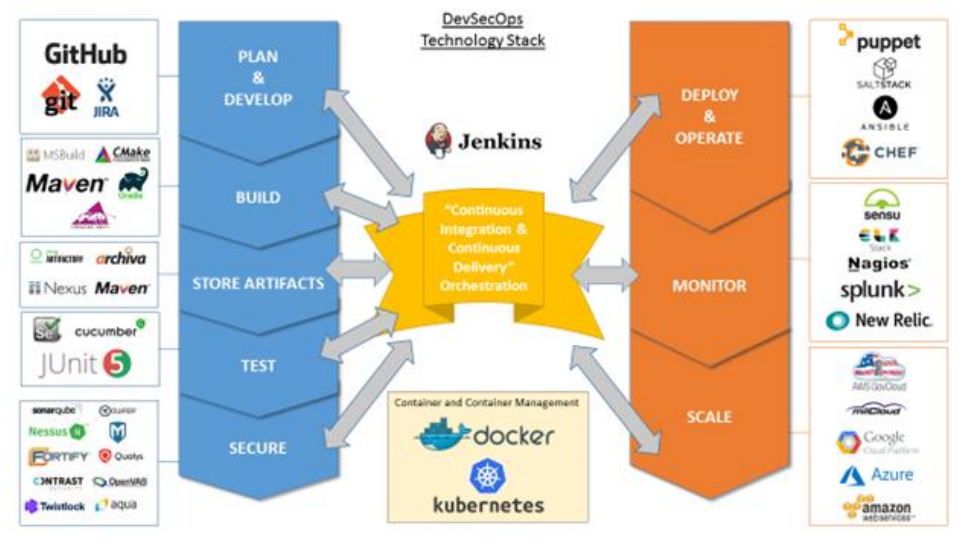
\includegraphics[width = .9\textwidth]{images/figure1.png}
\end{center}

\begin{paracol}{2}
    \begin{leftcolumn}
        Git, ClearCase, or Subversion - version control system for tracking changes to source code. Git is the de facto open source standard for modern software development.

        ...
    \end{leftcolumn}
    \begin{rightcolumn}
        Git, ClearCase,或者Subversion——用于跟踪源代码变更的版本控制系统。Git实际上是现代软件开发的开源标准。

        ...
    \end{rightcolumn}
\end{paracol}

\end{document}